\documentclass[main.tex]{subfiles}

\begin{document}

\section{Aufgabe 1}
Bei einer Klassenarbeit erhielten die $25$ Schülerinnen und Schüler einer Klasse in alphabetischer Reihenfolge die Zensuren
\begin{center}
$3$, $5$, $4$, $3$, $2$, $3$, $4$, $6$, $1$, $2$, $3$, $3$, $4$, $5$, $2$, $1$, $3$, $4$,	$2$, $4$, $3$, $1$, $2$, $3$, $4$
\end{center}
\begin{enumerate}
\item Erstellen Sie eine Tabelle mit Strichliste sowie absoluter und relativer Häufigkeit jeder Zensur. Zeichnen Sie ein Stabdiagramm der empirischen Häufigkeitsverteilung.
\item Ergänzen Sie die Tabelle um die Werte für die empirische Verteilungsfunktion und zeichnen Sie diese.
\item Berechnen Sie
\begin{enumerate}
\item das arithmetische Mittel
\item den Median
\item den Modalwert
\item das $10\%$-Quantil
\item das obere Quartil
\item die empirische Varianz und die empirische Standardabweichung
\end{enumerate}
\item Geben Sie den Variationskoeffizienten an.
\end{enumerate}

\subsection{Lösung 1}

\begin{center}
    \begin{tabular}{c|l|c|c|c}
        Zensur $A_j$ & Striche & Ereignisse $h_j$ & relative H. $r_j$ & kumulierte H. $H_j$ \\\hline
        1 & \StrokeThree            & 3 & 0,12 & 0,12 \\
        2 & \StrokeTwo              & 5 & 0,2  & 0,32 \\
        3 & \StrokeFive\StrokeThree & 8 & 0,32 & 0,64 \\
        4 & \StrokeFive\StrokeOne   & 6 & 0,24 & 0,88 \\
        5 & \StrokeTwo              & 2 & 0,08 & 0,96 \\
        6 & \StrokeOne              & 1 & 0,04 & 1,0 \\\hline
        $\sum$ & \StrokeFive\StrokeFive\StrokeFive\StrokeFive\StrokeFive & 25 & 1
    \end{tabular}
\end{center}

\begin{figure}[h]
    \begin{center}
        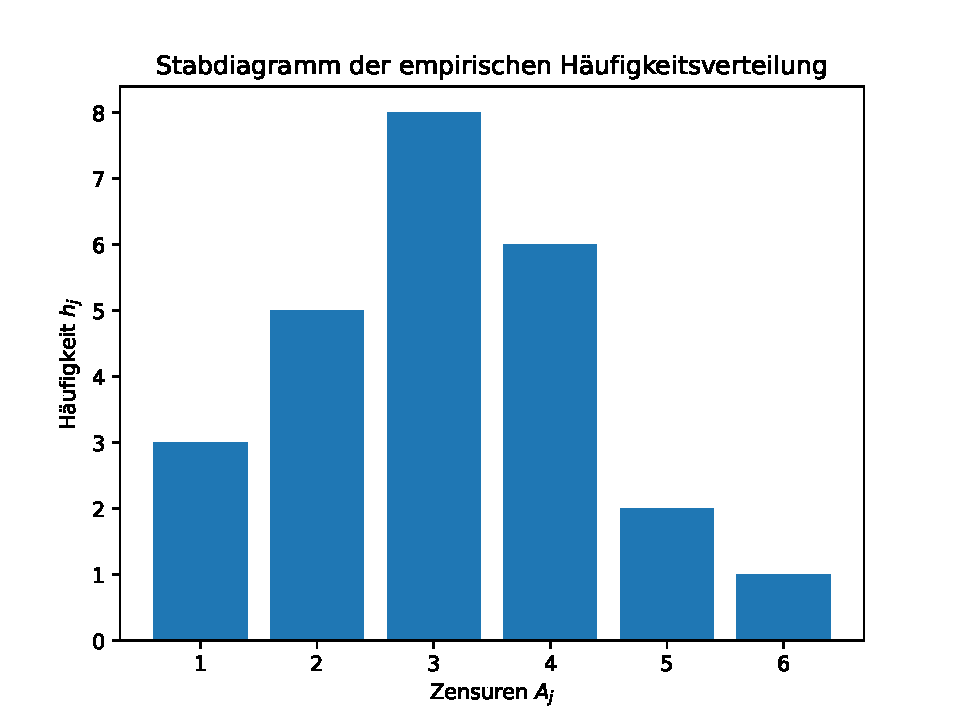
\includegraphics[width=0.7\textwidth]{A1-a.pdf}
        \caption{Lösung der Aufgabe 1a}
    \end{center}
\end{figure}

\begin{figure}[h!]
    \begin{center}
        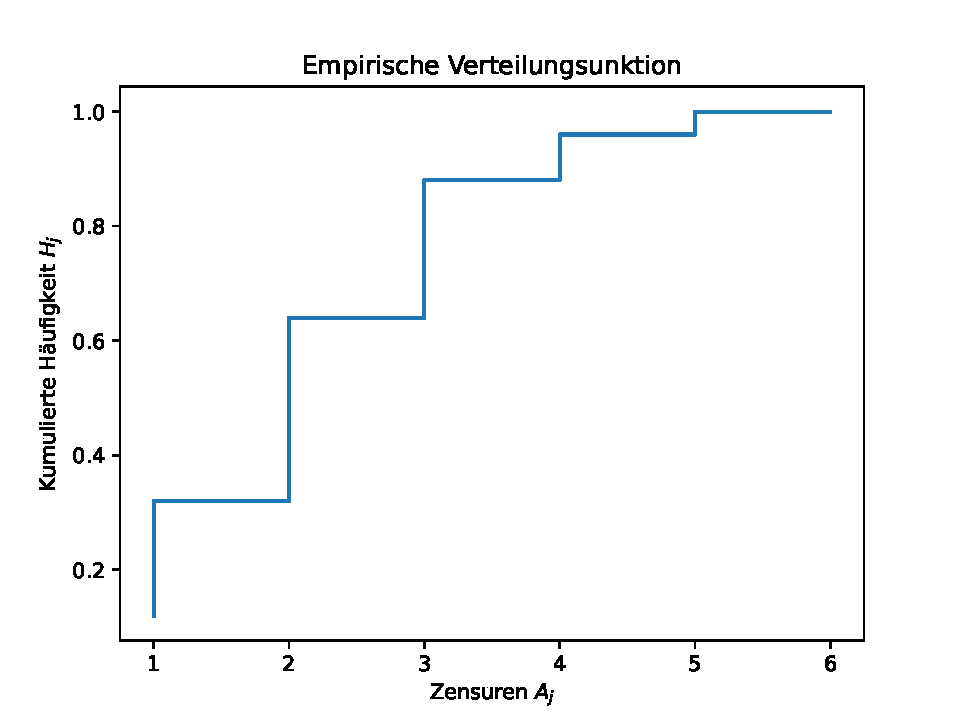
\includegraphics[width=0.7\textwidth]{A1-b.pdf}
        \caption{Lösung der Aufgabe 1b}
    \end{center}
\end{figure}
\renewcommand{\labelenumi}{\theenumi}
\renewcommand{\theenumi}{\roman{enumi}.}%
\begin{enumerate}
    \item Das arithmetische Mittel der Noten beträgt $\overline{x}=\frac{77}{25} = 3,08$
    \item Der Median (der mittlere Wert in einer geordneten Liste von Daten) der Noten ist 3,0
    \item Der Modalwert, also die am häufigsten vorkommende Note, ist 3.
    \item Das $10\%$-Quantil der Noten liegt bei $x_{(\lfloor 25 \cdot 0,1 + 1 \rfloor)} = x_{(3)} = 1$. Das bedeutet, dass 10\% der Noten unter diesem Wert liegen.
    \item Das obere Quartilliegt bei $x_{(\lfloor 25 \cdot 0,75 +1 \rfloor)} = x_{(19)} = 4$. Das bedeutet, dass 75\% der Noten unter oder gleich diesem Wert sind.
    \item Die empirische Varianz beträgt $s^2 = 1,66$ und die empirische Standardabweichung $s \approx 1,288$.
\end{enumerate}

Der Variationskoeffizienten $V$, drückt das Verhältnis der Standardabweichung zum Mittelwert aus und ist ein Maß für die relative Streuung der Daten.
$$
    V = \frac{s}{\overline{x}} = 0,41831
$$

\end{document}
